\documentclass[10pt,conference,compsocconf]{IEEEtran}
\usepackage{graphicx}
\usepackage{subfigure}
\usepackage{multirow}
\usepackage{balance}
\usepackage{blindtext}
\usepackage{comment}
\usepackage{algorithm}
\usepackage{algpseudocode}
\usepackage{pifont}
\usepackage[justification=centering]{caption} %% for centering the caption
\usepackage[belowskip=-5pt,aboveskip=10pt]{caption} %for the blank above and below caption
% correct bad hyphenation here
\hyphenation{op-tical net-works semi-conduc-tor}


\begin{document}
%
% paper title
% can use linebreaks \\ within to get better formatting as desired
\title{Tentative: Improving big data processing at large scale on supercomputers using multithreading and advanced MPI features }


% author names and affiliations
% use a multiple column layout for up to three different
% affiliations


\author{ \IEEEauthorblockN{Boyu Zhang\IEEEauthorrefmark{1}, Wesley 
    Bland\IEEEauthorrefmark{2}, Pavan Balaji\IEEEauthorrefmark{3},
    Michela Taufer\IEEEauthorrefmark{1}}
  \IEEEauthorblockA{\IEEEauthorrefmark{1}University of Delaware
    \\\{bzhang, taufer\}@udel.edu}
  \IEEEauthorblockA{\IEEEauthorrefmark{2}Intel Corporation
    \\wesley.bland@intel.com}
  \IEEEauthorblockA{\IEEEauthorrefmark{3}Argonne National Laboratory
     \\balaji@anl.gov} }

% make the title area
\maketitle

\begin{abstract}
%\boldmath
NA.
\end{abstract}

% IEEEtran.cls defaults to using nonbold math in the Abstract.
% This preserves the distinction between vectors and scalars. However,
% if the conference you are submitting to favors bold math in the abstract,
% then you can use LaTeX's standard command \boldmath at the very start
% of the abstract to achieve this. Many IEEE journals/conferences frown on
% math in the abstract anyway.

% no keywords
% For peer review papers, you can put extra information on the cover
% page as needed:
% \ifCLASSOPTIONpeerreview
% \begin{center} \bfseries EDICS Category: 3-BBND \end{center}
% \fi
%
% For peerreview papers, this IEEEtran command inserts a page break and
% creates the second title. It will be ignored for other modes.
\IEEEpeerreviewmaketitle

\section{Introduction}
\label{introduction}

The goal of this work is to bridge big data processing on HPC platforms 
such as supercomputers. MapReduce model provides an easy way for
application programmers to deal with distributed big data. Moreover,
there exist many runtime libraries that support MapReduce on cloud
environment such as hadoop etc. At the same time, HPC platforms such
as supercomputers provides high performance computation (multicore per node),
 communication (MPI), and storage capabilities (high performance shared
 file system such as lustre).

Some research effort targets to bridge big data processing
on HPC platforms such as supercomputers. This is important due to
the fact that many scientific applications (e.g. xx, yy) run on HPC platforms,
they generate big data that need to be processed in an in-situ or in-transit manner
(cite xx). MapReduce-MPI is a popular framework that enables big data
on HPC platforms. However, MRMPI has poor performance at large
scale. Figure xx shows for benchmark word count and clustering,
when using 2048 computing cores, the weak scalability is bad due to
the long shuffle time that involves all to all communications. The root
of the poor performance is two design choices: (1) MRMPI uses a process-based
model. Each MPI process runs map and reduce functions. To take advantage
of multiple computing cores per node, one needs to run multiple MPI
processes per node. This results in communication happens 
from process to process, hence multiple communication channels established
among two nodes which in fact only 1 is needed. (2) MRMPI uses blocking
MPI\_Alltoallv to do the all to all communication in the shuffling stage. This
precludes the possibility of overlapping communication and computation
in the process. These two design choices increase the number of
processes involved in the all to all communication, and block computation
while communication is undergoing. 

In our new design, we overcome these two disadvantages by using:
(1) a hybrid MPI process and multithreaded based model. Each MPI
process runs multithreaded version of map and reduce functions. One
can take advantage of multiple computing cores per node by running
one process on each node, and running multithreaded map and reduce
functions per node. This reduce the number of process involved in the
all to all communication, ensures that the communication happens 
among nodes, which is the minimum communication size; (2) non-blocking
MPI\_Ialltoallv communication which is available since MPI version xx.
This allows overlapping of communication with map computation.

The evaluation using benchmarks show that our new MapReduce
model improves the performance at large scale.

This paper makes three significant contributions:
\begin{itemize}
\item It presents a MapReduce runtime library using multithreaded 
design and advanced MPI features.
\item It improves the scalability of big data processing on supercomputers
at large scale.
\item It shows ...
\end{itemize}

The rest of this paper is organized as follows:
Section~\ref{s:related_work} reviews the related work on trajectory
analysis and distributed big data analytics; Section~\ref{s:method}
presents our method in detail; Section~\ref{s:validation} shows the
validation of the method using statistical and empirical techniques;
Section~\ref{s:implementation} discusses the implementation aspects in
Parallel MATLAB; Section~\ref{s:evaluation} presents the performance
evaluations; and Section~\ref{s:conclusions} concludes the paper and
gives directions for future work.







\section{Background}
\label{background}
\subsection{MapReduce programming model and runtime libraries}
\begin{itemize}
\item map, shuffle, reduce stages, automatically run in parallel
\item MapReduce-MPI, map, s, r run sequentially, c++ and mpi
\item Hadoop
\end{itemize}

In a typical MapReduce runtime library such as MapReduce-MPI, the library
implements three major phases: map, shuffle, and reduce, as shown in 
Figure~\ref{fig:overview_mtmr}(a). Map phase reads the initial input and
emits the intermediate $\langle key, value \rangle$ pairs. Shuffle phase communicates
all the $\langle key, value \rangle$ pairs with the same key to the same process
and forms the key and list of values as the input to reduce function. Reduce
phase applies reduce function to all the values associated with the
same key and output final results.

MapReduce-MPI is a runtime library written in C++ and MPI that
enables MapReduce operations on HPC platforms.
\begin{itemize}
\item mrmpi runs map and reduce function in an individual process.
\item map, read input, apply map function, output intermediate 
output to disk files
\item communication, after map is done on all processes, 
mpi alltoallv
\item reduce, after communication is done, apply reduce.
\end{itemize}

\subsection{Non-blocking MPI collectives}
discuss the blocking MPI\_Alltoallv vs. non-blocking MPI\_Ialltoallv.
syntax of mpi ialltoallv

\section{The MTMR system}
MTMR implements MapReduce for traditional HPC systems such as 
supercomputers. Its goal is to enable efficient big data processing
at large scale.


\subsection{MTMR runtime design}

The MTMR is developed using C++, MPI, and OpenMP. It uses OpenMP to
enable multithreaded processing in map and reduce functions. It uses 
non-blocking MPI collectives to communicate $\langle key, value \rangle$ pairs 
between map and reduce phases, and to overlap communication
with map computation. 

With the goal of optimizing the shuffle stage performance,
there are two main design choices that we used. First, our library adapted
a multithreaded model for map and reduce functions. Second, 
we used non-blocking MPI collectives to overlap communication
and computation. We briefly introduce them here and discuss them in
details in the following sessions.

Comparing to the MapReduce-MPI which runs one MPI process
on each computing core, our library runs one MPI process on each
computing node, and uses OpenMP to take advantage of intra-node
parallelism. The reasoning behind this decision is to improve
the performance of the all-to-all communication in the shuffle stage.
As shown in Figure~\ref{}, the performance of the MPI\_Alltoallv 
is improved in the case of using one process on each node than 
using one process on each core when communicating the same
amount of data that follows the same node-to-node communication
pattern. To use MPI\_Alltoallv more efficiently, we adopt this one
process per node pattern, and use multiple threads to execute map
and reduce functions.

Moreover, with the support of non-blocking collective in MPI, it
enables library writers to overlap communication and computation 
easily. Our library starts communicating $\langle key, value \rangle$ pairs 
as soon as the first memory buffer which stores the the $\langle key, value \rangle$
pairs is full, this allows our system to overlap communication
and computation efficiently.

Figure~\ref{overview_mtmr} shows the comparison of our 
Multithreaded MapReduce library with the MapReduce-MPI library.
As discussed in Section~\ref{background}, the shuffle stage
can be divided into two steps: communication and reorganization. The 
communication step sends and receives $\langle key, value \rangle$  pairs. 
The reorganization step gathers all the values associated with
the same key (the values may come from different processes) and 
forms the input to reduce. 
n MapReduce-MPI, the
shuffle phase starts after the map phase, and finishes before the
reduce phase. In comparison, our library pushes the communication
step of the shuffle into the map phase, and combines the reorganization
step with the reduce phase.
\begin{figure}[!htb]
\centering
  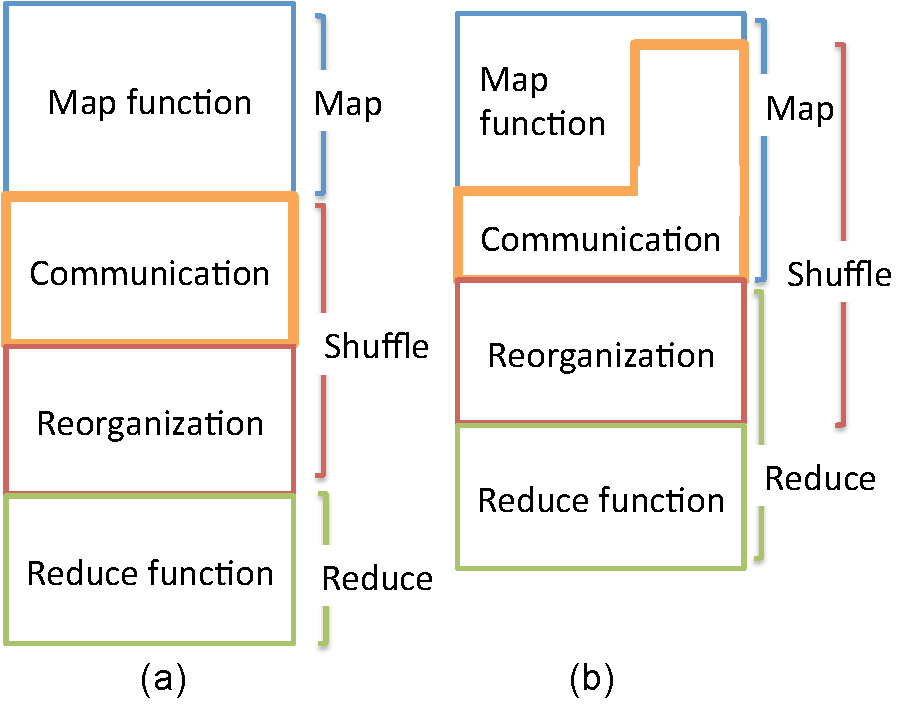
\includegraphics[width=0.9\linewidth,height=2.2in]{figs/overview_mtmr.pdf}
  \caption{MapReduce operations: map, shuffle, and reduce operations in a
  typical MapRedue runtime such as MapReduce-MPI (a); and map, shuffle, and
  reduce operations in our MTMR runtime (b).}
  \label{fig:overview_mtmr}
\end{figure}

\subsection{Design of multithreaded map}

Key points:
\begin{itemize}
\item double buffers for (1) work sharing among threads (2) non-blocking 
communication
\item how to handle thread synchronization when using double buffers,
use atomic fetch and add operation, use local buffer per thread
\item improvements and advantages over MRMPI (or Hadoop)
\end{itemize}

The overall process of map is presented in Figure~\ref{fig:multithreaded_map}.  
The map process reads initial input into a memory buffer and stores them as
data records. We denote the memory buffer which stores the
data records by $BUFF_{input}$. The input can be broken up into records
in multiple ways. Currently, our library supports two types of
data records. In the first type, each data record is a English
word; while in the second type, each data record is one line
of text in the input.
\begin{figure*}[!htb]
\centering
  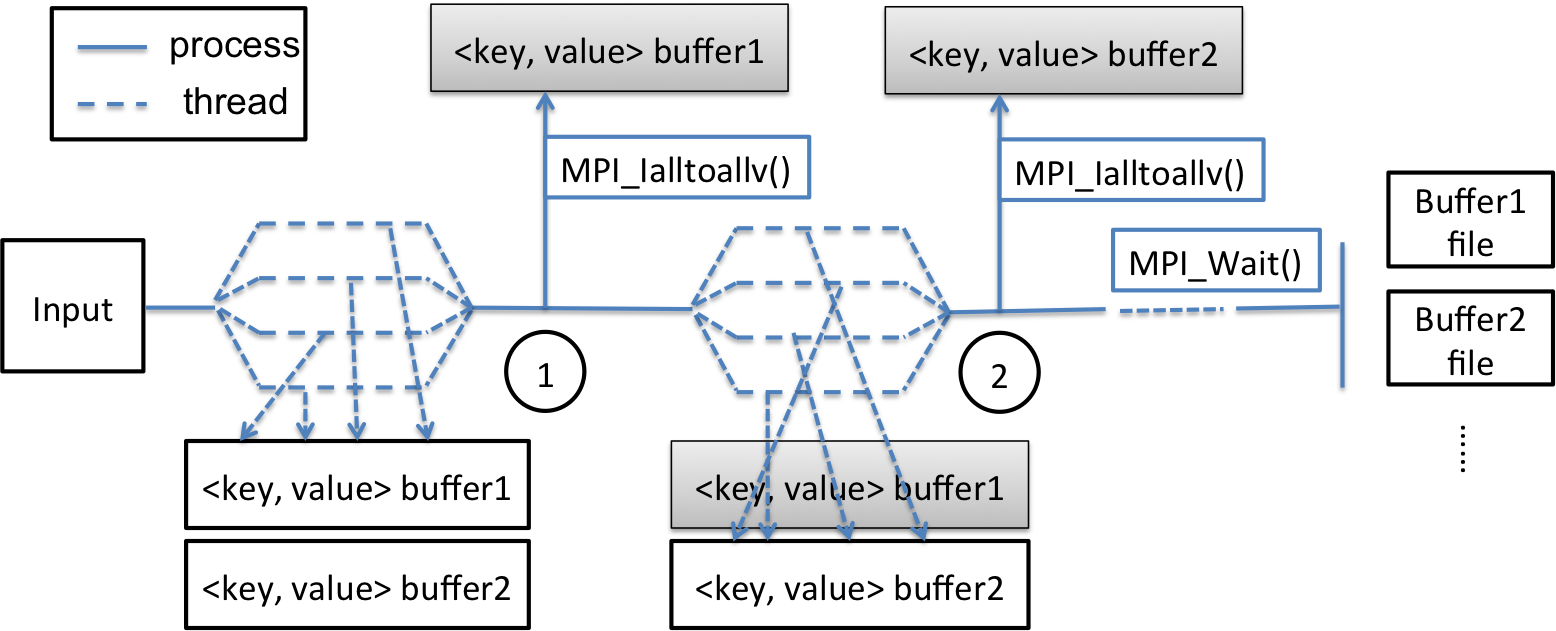
\includegraphics[width=0.8\linewidth,height=2.2in]{figs/multithreaded_map_design.png}
  \caption{Design of multithreaded Map phase.}
  \label{fig:multithreaded_map}
\end{figure*}

When the $BUFF_{input}$ is full, the process starts an 
OpenMP session in which
each thread reads a subset of data records from the $BUFF_{input}$, applies the user
defined map function to each record, generates
the intermediate $\langle key, value \rangle$ paris, and stores the intermediate
$\langle key, value \rangle$ pairs collectively into a second memory.
We denote the second memory buffer by $BUFF_{kv1}$.
$BUFF_{kv1}$ is used for two purposes. First, it stores
the intermediate output for each map process. Second,
it is used as the send buffer in the subsequent MPI\_Ialltoallv()
to communicate the intermediate data.

There are two important aspects that we need to consider.
First, in order to use $BUFF_{kv1}$ as the send buffer in MPI\_Ialltoallv(),
all the intermediate pairs that need to be sent to process $p_{i}$ need
to be stored in a continuous region. To this end, we partition
the $BUFF_{kv1}$ into n regions of the same size, n is the number
of process running. Then we apply a hash function to determine
the destination process of the intermediate pair and store
the pair in corresponding region of $BUFF_{kv1}$. 
We use an additional array to keep track of location in $BUFF_{kv1}$
to store the next pair. Figure~\ref{fig:map_data_structures}(a) shows
the $BUFF_{kv1}$ after partition when there are four processes,
and Figure~\ref{fig:map_data_structures} shows the corresponding OFFSET array
that stores the location to write the next intermediate pair.
\textbf{write something about the hash function, give ref}
\begin{figure}[!htb]
\centering
  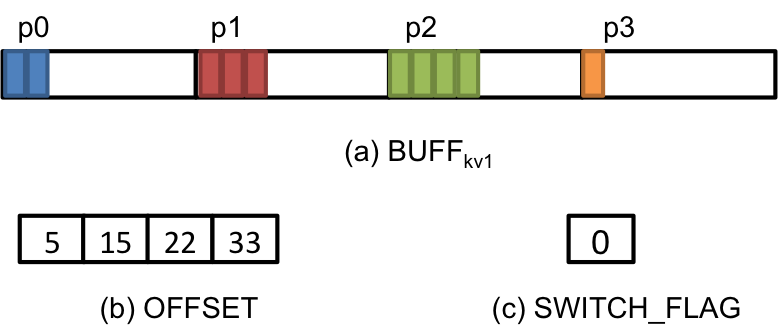
\includegraphics[width=0.9\linewidth,height=1.2in]{figs/map_data_structures.png}
  \caption{MapReduce operations: map, shuffle, and reduce operations in a
  typical MapRedue runtime such as MapReduce-MPI (a); and map, shuffle, and
  reduce operations in our MTMR runtime (b).}
  \label{fig:map_data_structures}
\end{figure}

Second, in order to avoid data race when multiple threads
try to write to the same buffer location,  and to ensure all threads exit
the parallel session in case any section of the $BUFF_{kv1}$ overflows, 
we need to ensure efficient synchronization. To this end, 
we use atomic operation $fetch\_and\_add$ as shown in
Algorithm~\ref{ag:sync_map}, and
a boolean variable named SWITCH\_FLAG as shown in 
Figure~\ref{fig:map_data_structures}(c).
$SWITCH\_FLAG  = false$ means it is OK to write the current
intermediate pair to $BUFF_{kv1}$ without overflowing it. Otherwise,
it means writing the current pair will overflow $BUFF_{kv1}$, and 
all threads should exit the parallel session, and $BUFF_{kv1}$ 
needs to be communicated using MPI\_Ialltoallv().
\begin{algorithm}
\caption{Synchronization in Multithread Map}
\label{ag:sync_map}
\begin{algorithmic}[1]
\While{$left > 0$}
\State \#pragma opm parallel
\State \{
\While{  $left_{me} > 0$ \&\& $!SWITCH\_FLAG$}
\State $\langle key, value \rangle \gets map(record)$
\State $offset \gets fetch\_and\_add(\&offset[i], size)$
\If{$offest + size < limit$}
\State copy $\langle key, value \rangle$ to $BUFF_{kv1}$
\State $myDone\mathrel{++}$
\Else
\State $SWITCH\_FLAG = true$
\EndIf
\EndWhile
\State \}
\State \#pragma omp atomic
\State $left \mathrel{-}= myDone$
\EndWhile
\end{algorithmic}
\end{algorithm}

In Algorithm~\ref{ag:sync_map}, $left$ is the number of data record
that need to be processed in $BUFF_{input}$. When there exists 
some data records need to be processed, we start a parallel session.
Each thread keeps track of the number of data record it needs to
process (local variable $left_{me}$), and reads the value of SWITCH\_FLAT
which is a global variable. If the both conditions are met, i.e., the
thread has some number of data records to process, and the
$BUFF_{kv1}$ is not overflowed, the thread calls the user
defined map function, reserves storage space in the $BUFF_{kv1}$
by calling $fetch\_and\_add$. The it tests to see if by copying 
the intermediate pair will overflow the $BUFF_{kv1}$, if not,
the intermediate pair is copied to $BUFF_{kv1}$, otherwise,
the overflow buffer flag $SWITCH\_FLAG$ is set to true.

We can validate the correctness of this algorithm by considering
the following scenarios. Hypothetically, we have four processes
in the system, and each process runs two threads (i.e. $T0$ and $T1$). The following 
four scenarios cover all possible execution paths that may
cause a data race or a buffer overflow. Due to space limitation,
we list the scenarios here, and leave the details of walking through 
the algorithm to the readers.

\begin{itemize}
\item Two threads try to write to different sections of $BUFF_{kv1}$,
$T0$ overflows the buffer, and $T1$ does not.
\item Two threads try to write to different sections of $BUFF_{kv1}$,
both overflow the buffer.
\item Two threads try to write to same sections of $BUFF_{kv1}$,
$T0$ overflows the buffer, and $T1$ does not.
\item Two threads try to write to same sections of $BUFF_{kv1}$,
both overflow the buffer.
\end{itemize}

We realize that the frequent calls to the atomic
$fetch\_and\_add$ is the bottleneck for performance and apply
further optimization by introducing a thread local memory
buffer to hold intermediate $\langle key, value \rangle$ pairs.
The thread local memory buffer has a similar structure as
shown in Figure~\ref{fig:mao_data_structures}(a), but much
smaller in size (\textbf{give numbers}). Each thread writes
to its local buffer first without the need to use atomic
operations, only when its local buffer overflows, the thread
calls $fetch\_and\_add$ to reserve space in the process 
owned global buffer $BUFF_{kv1}$. The process requires 
only minor changes to Algorithm~\ref{ag:syn_map}. 

Continue with the map processing, after having enough 
intermediate pairs that eventually make $BUFF_{kv1}$ overflow,
the threads exit the parallel session collectively. At this point,
the process communicates the $BUFF_{kv1}$ using 
non-blocking $MPI\_Ialltoallv()$, and immediately continues to process 
data records in $BUFF_{input}$ that are left.
This time, the threads stores intermediate pairs in a third 
memory buffer named $BUFF_{kv2}$ as shown in Figure~\ref{fig:multithreaded_map}.
This operation of multithreaded mapping and storing intermediate
data to a memory buffer (either $BUFF_{kv1}$ or $BUFF_{kv2}$), and
communicating of the full memory buffer among processes
repeat until all the input files are exhausted. The we
wait for all the previous $MPI\_Ialltoallv()$ to return using $MPI_Wait()$
before moving on to the reduce phase. 
 
The use of double buffering serves both purposes of working sharing
among threads, and the send buffer for communication. It 
brings several merits including


The key idea of the design is to use one process on each node to ensure
node to node communication (instead of multiple communication channels
among two nodes), and to use multiple threads to apply the map function
to generate the intermediate key value pairs. To enable the design, we 
use two buffers (double buffer, overflow buffer?) to hold intermediate 
key value pairs for the direct communication among processes (nodes), without
spilling on disk file (which is the case of MR-MPI).

In the map function, the process first reads the input
file into the memory buffer \textit{in\_buffer}, (called \textit{in\_buffer}, size is configureable 
by the user). At the same time, each process
maintains two memory buffers (named \textit{kv\_buffer1} and \textit{kv\_buffer2}) 
to store the intermediate output of map function. After the \textit{in\_buffer} is
populated with data records, the program spawns an OpenMP parallel
session, in which each thread reads a distinct part of the data records
in \textit{in\_buffer}, applies the user defined map function, and writes the
intermediate output to the \textit{kv\_buffer} collectively. When the 
\textit{kv\_buffer} is full, it is used as the MPI send buffer in the non-blocking
MPI\_Ialltoallv communication to send key value pairs. 

---

The benefits are:


\subsection{Multithreaded reduce}

Key point:
\begin{itemize}
\item almost entirely multithreaded
\item use dictionary and hash table to reorganize 
\end{itemize}

The use of dictionary and hash table are suggested by yanfei, need to point out.
The reduce phase is almost entirely multithreaded. The reduce phase starts
by reorganizing the $\langle key, value \rangle$ pairs received in one buffer to group
all the values associated with the same key. Then the reduce phase
reorganizes the pairs across all the buffers received from the map phase.







\section{Evaluation}
\label{s:evaluation}

\subsection{Platform and benchmarks}


\subsection{Performance results }





\section{Related Work}
\label{s:related_work}

this and that



\section{Conclusion and future work}
\label{s:conclusions}

In this paper, we presented a method to study intra- and
inter-trajectory analysis in large protein-folding datasets on
distributed memory systems. Our method is a one-pass, distributed
process that is efficient and suitable for in-situ data analysis:
it avoids the need for moving trajectory data, uses a limited amount of 
memory, and is faster than traditional approaches.
We implemented the method in a modular framework using
Parallel MATLAB and evaluated its performance using the folding
trajectory of the protein HP-35 NleNle (i.e., a variant of the villin
headpiece subdomain) on 256 compute cores of Gordon supercomputer. 
We compared our method's performance with a more traditionally used,
centralized approach and observed significantly faster runtimes
(i.e., two orders of magnitude faster, 41.5 seconds comparing to 3
hours in the traditional method). We also observed a three and four
orders of magnitude reduction respectively in the size of data
movement and memory usage (i.e., 6.9 MB memory usage comparing to 16
GB in the traditional method, 4.4 KB data moved comparing to 539
MB). In addition, our method presents a linear weak scalability and
maintains a parallel efficiency above 90\% when using up to 128
cores. 

Future work includes testing the accuracy and scalability of our method for 
larger datasets of protein-folding trajectories containing more diverse
protein conformations (i.e., alpha-helix and beta-sheet) than the
villin subdomain and for larger distributed memory systems. We are also 
committed to closely work with domain scientists to
explore the benefit of our method to the study of the protein-folding
process.

\balance


% use section* for acknowledgement
\section*{Acknowledgment}
This work is supported in part by NSF grants: DMS 0800272/0800266, and CCF-SHF 1318445/1318417. This work used the Extreme Science and Engineering Discovery Environment (XSEDE), which is supported by National Science Foundation grant number OCI-1053575. The authors want to thank Dr. Vijay Pande and T. J. Lane from Stanford  for providing us with the dataset for our tests. All the software will be made available before the conference. 




\balance


% use section* for acknowledgement
\section*{Acknowledgment}
This work is supported in part by NSF grants: DMS 0800272/0800266, and CCF-SHF 1318445/1318417. This work used the Extreme Science and Engineering Discovery Environment (XSEDE), which is supported by National Science Foundation grant number OCI-1053575. The authors want to thank Dr. Vijay Pande and T. J. Lane from Stanford  for providing us with the dataset for our tests. All the software will be made available before the conference. 

%\newpage
% trigger a \newpage just before the given reference
% number - used to balance the columns on the last page
% adjust value as needed - may need to be readjusted if
% the document is modified later
%\IEEEtriggeratref{8}
% The "triggered" command can be changed if desired:
%\IEEEtriggercmd{\enlargethispage{-5in}}

% references section

% can use a bibliography generated by BibTeX as a .bbl file
% BibTeX documentation can be easily obtained at:
% http://www.ctan.org/tex-archive/biblio/bibtex/contrib/doc/
% The IEEEtran BibTeX style support page is at:
% http://www.michaelshell.org/tex/ieeetran/bibtex/
%\bibliographystyle{IEEEtran}
% argument is your BibTeX string definitions and bibliography database(s)
%\bibliography{paper}
%
% <OR> manually copy in the resultant .bbl file
% set second argument of \begin to the number of references
% (used to reserve space for the reference number labels box)
%\begin{thebibliography}{11}
%
%\bibitem{IEEEhowto:kopka}
%H.~Kopka and P.~W. Daly, \emph{A Guide to \LaTeX}, 3rd~ed.\hskip 1em plus
%  0.5em minus 0.4em\relax Harlow, England: Addison-Wesley, 1999.
%
%\end{thebibliography}

% Generated by tran.bst, version: 1.13 (2008/09/30)
%\small
\begin{thebibliography}{10}
%\providecommand{\url}[1]{#1}
%\csname url@samestyle\endcsname
%\providecommand{\newblock}{\relax}
%\providecommand{\bibinfo}[2]{#2}
%\providecommand{\BIBentrySTDinterwordspacing}{\spaceskip=0pt\relax}
%\providecommand{\BIBentryALTinterwordstretchfactor}{4}
%\providecommand{\BIBentryALTinterwordspacing}{\spaceskip=\fontdimen2\font plus
%\BIBentryALTinterwordstretchfactor\fontdimen3\font minus
%  \fontdimen4\font\relax}
%\providecommand{\BIBforeignlanguage}[2]{{%
%\expandafter\ifx\csname l@#1\endcsname\relax
%\typeout{** WARNING: tran.bst: No hyphenation pattern has been}%
%\typeout{** loaded for the language `#1'. Using the pattern for}%
%\typeout{** the default language instead.}%
%\else
%\language=\csname l@#1\endcsname
%\fi
%#2}}
%\providecommand{\BIBdecl}{\relax}
%\BIBdecl

\bibitem{Phillips2011} J.~Phillips et al., ``Validating clustering of
  molecular dynamics simulations using polymer models,'' \emph{BMC
    Bioinformatics}, vol.~12, no.~1, pp. 445--467, 2011.  
\bibitem{Tu2008} T.~Tu et al., ``A scalable parallel framework for
  analyzing terascale molecular dynamics simulation trajectories,'' in
  \emph{Proc. of the 2008 ACM/IEEE International Conference for High
    Performance Computing, Networking, Storage and Analysis (SC'08)}, pp. 1--12, 2008.
\bibitem{Best2002} C.~Best and H.~C. Hege, ``Visualizing and
  identifying conformational ensembles in molecular dynamics
  trajectories,'' \emph{Computing in Science Engineering}, vol.~4,
  no.~3, pp. 68--75, 2002.
\bibitem{bigdataweb} M. Stonebraker. (2012, Sept. 21). What does big
  data mean [ONLINE]. Available:
  http://cacm.acm.org/blogs/blog-cacm/155468-what-does-big-data-mean/fulltext
\bibitem{Bennett2012} J.~C. Bennett et al., ``Combining in-situ and
  in-transit processing to enable extreme-scale scientific analysis,''
  in \emph{Proc. of the 2012 ACM/IEEE International Conference for
    High Performance Computing, Networking, Storage and Analysis
    (SC'12)}, pp. 1--9, 2012.
\bibitem{Lakshminarasimhan2013} S.~Lakshminarasimhan et al.,
  ``Scalable in-situ scientific data encoding for analytical query
  processing,'' in \emph{Proc. of the 22nd International Symposium on
    High-performance Parallel and Distributed Computing (HPDC '13)}, pp. 1--12, 2013.
\bibitem{Cordeiro2011} R.~L.~F. Cordeiro et al., ``Clustering very
  large multi-dimensional datasets with {MapReduce},'' in
  \emph{Proc. of the 17th ACM SIGKDD International Conference on
    Knowledge Discovery and Data Mining (KDD'11)}, pp. 690--698, 2011.
\bibitem{Liu2013} J.~Liu et al., ``Segmented analysis for reducing
  data movement,'' in \emph{Proc. of the IEEE International conference
    on Big Data (BigData'13)}, 2013.
\bibitem{Pande2007} D.~L. Ensign et al., ``Heterogeneity even at the
  speed limit of folding: large-scale molecular dynamics study of a
  fast-folding variant of the villin headpiece,'' \emph{Journal of
    Molecular Biology}, vol.  374, no.~3, pp. 806--816, 2007.
\bibitem{Borg2009} I.~Borg and P.~J.~F. Groenen, \emph{Modern
  multidimensional scaling: theory and applications}, Springer, 2005.
\bibitem{FCM} R.~L. Cannon et al., ``Efficient implementation of the
  fuzzy c-means clustering algorithms,'' \emph{IEEE Transactions on
    Pattern Analysis and Machine Intelligence}, vol.~8, no.~2,
  pp. 248--255, 1986. 
    \bibitem{Mooi2011} E.~Mooi and M.~Sarstedt, ``Chapter 9 -
      clustering analysis", in \emph{A Concise Guide to Market
        Research: The Process, Data, and Methods Using {IBM} {Spss}
        Statistics}, Springer, 2011.  
\bibitem{pearson} G.~W. Snedecor and W.~G. Cochran, ``The sample
  correlation coefficient {R}", in \emph{Statistical Methods}, 7th
  ed. Iowa State Press,1980.
  \bibitem{Moler1995} C.~Moler, ``Why there isn't parallel {MATLAB},''
    \emph{Mathworks Newsletter}, vol.~00, pp. 1--12, 1995.
\bibitem{Moler2013} C. Moler, ``Parallel {MATLAB}: {from hell no to
  you bet},'' \emph{Thirty Years of Parallel Computing at Argonne: A
  Symposium}, May 2013.
\end{thebibliography}

%[Total times in seconds across processes broken down into distinctive components: Map (M), Shuffle (S), Overhead (O), Reduce (R), and Total (T).]
%This is the appendix.


% that's all folks
\end{document}



% LocalWords:  priori
